For this event type, full-scale floor loads are generated by a web service, 
\href{http://evovw.ce.nd.edu/DEDM_HRP/DEDMP_INT_v3_4evo.html}{DEDM HRP} a Database-Enabled Design module 
for High-Rise buildings using Pressure data. The loads  are downloaded and then applied to the 
building when either of the run buttons are pressed.

To understand the inputs, it is necessary to understand that the DEDM-HRP website itself 
utilizes the aerodynamic database compiled at the Tokyo Polytechnic 
University, Japan (referred to simply as TPU database). THE TPU database contains data 
for a variety of building  configurations of different building width (B), depth (D), and 
height (H) ratios (B:D:H ratios), tested for various incident wind direction and exposure conditions.
 The TPU database comprises a total of 394 test cases, derived for 3 square/rectangular cross-sectional 
shapes, 4 to 5 model heights, 1 to 2 exposure categories and 11 to 21 incident wind directions of 5 
degree increments. 

\begin{figure}[!htbp]
  \centering {
    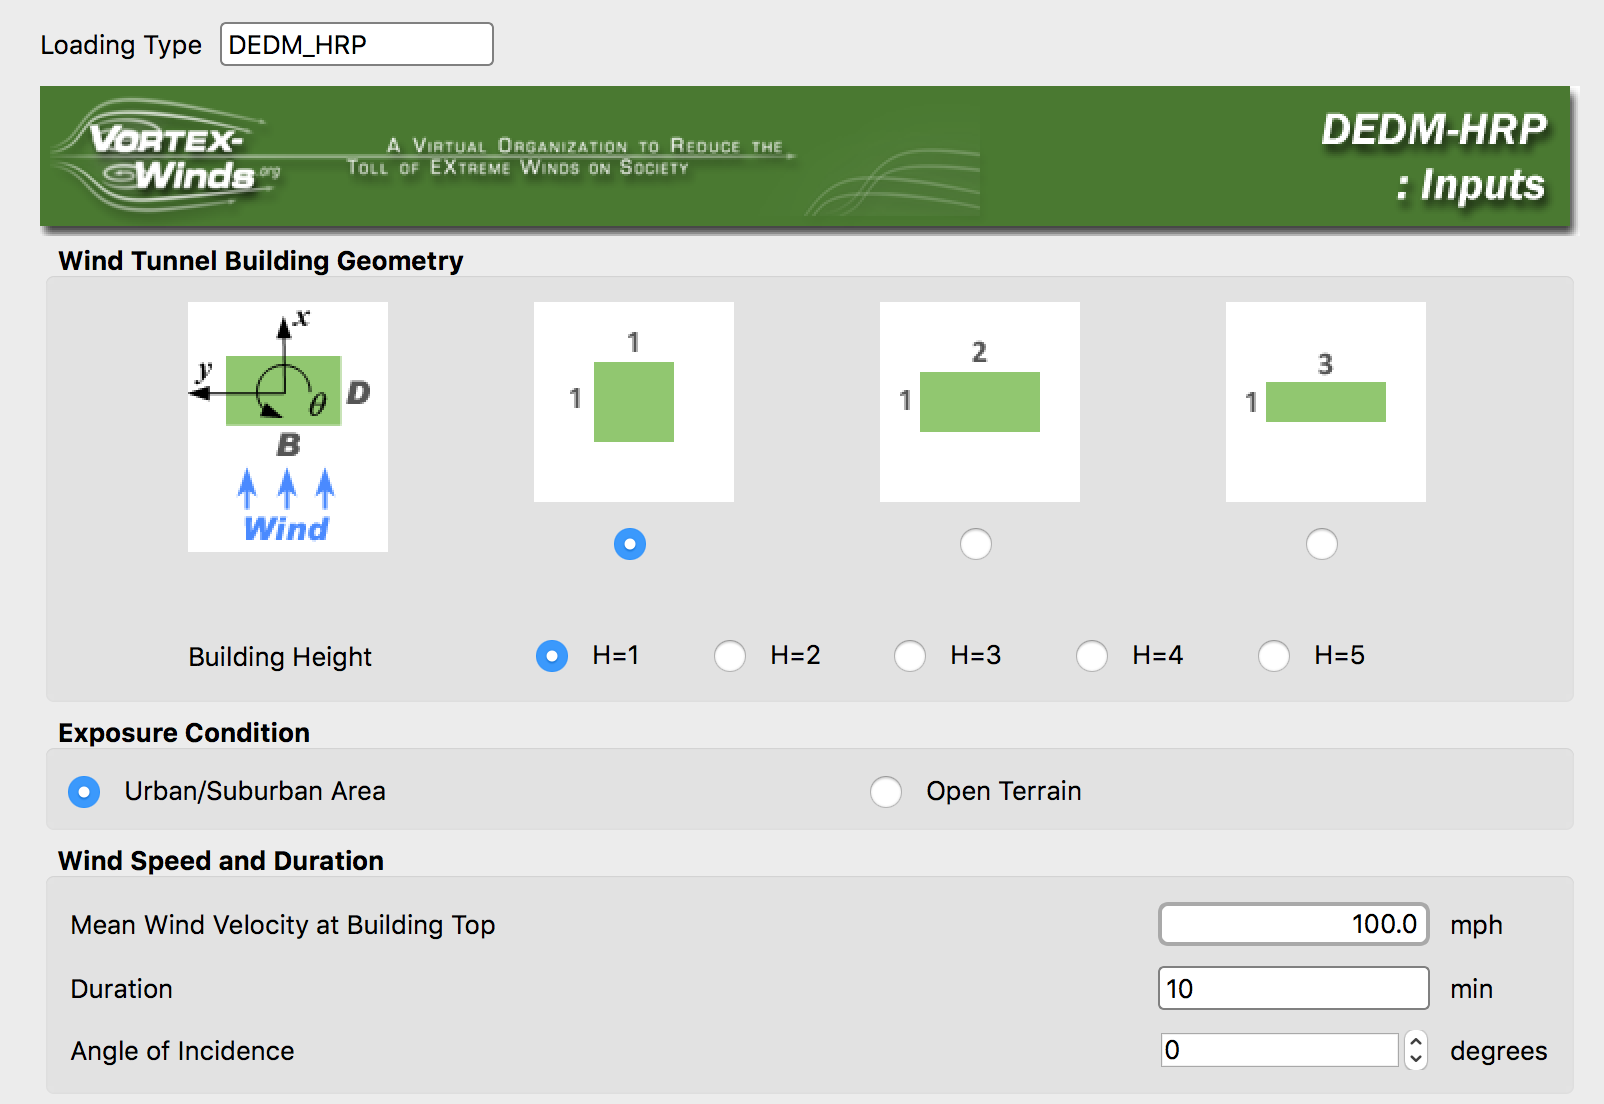
\includegraphics[width=0.8\textwidth]
    {usage/figures/dedmHRP.png} }
  \caption{DEDM HRP Wind Loading Event}
  \label{fig:dedm_hrp}
\end{figure}

In the inputs for the event, as shown in figure \Cref{fig:dedm_hrp} require the user to specify which 
of these tests to use:
\begin{enumerate} 
\item The user to select from one of the three cross sectional shapes.
\item The user specifies one of five building heights.
\item One of two exposure conditios: urban/suburban terrain (alpha = 0.25)
and open terrain (alpha = 0.167), which would correspond to Exposure B and C, respectively, 
as defined in ASCE 7 standard.
\item Mean Wind Speed at Top of Building: The basic wind speed in the ASCE standard 
(e.g., ASCE 7-16) is defined as 3-sec gust at 10 m height. However, the DEDM-HRP asks
the inputs of mean wind speeds at the top of a full-scale building. This is because of 
the nature of the TPU database: TPU’s pressure coefficients were obtained using mean wind 
speed at the top of a test model.
\item Duration of test data, either 10min or 1 hour.
\item The angle of incidence, 0 through 90 in 5 degree increments.
\end{enumerate}

The actual loads applied to the building that are obtained using the pressure taps. They are scaled from the TPU datasets based on the height of the building provided in the general information. The scaling employed by Vortex-Winds does not take into account the width and depth provided in the General Information. The forces are determined based on widths and depths of the wind tunnel model scaled by the height in the General Information to the height of the model in the wind tunnel experiment.

For details on \texttt{DEDM HRP}, the user is recomended to read the following:
Seymour M.J. Spence, Ahsan Kareem
Dae Kun Kwon, Seymour M.J.Spence, and Ahsan Kareem, ``A cyberbased Data-Enabled Design framework for high-rise buildings driven by synchronously measured surface pressures'', Advances in Engineering Software 2014, DOI:10.1016/j.advengsoft.2014.07.001


For this event, the wind speed can be a random variable.

